\documentclass[13pt, twoside, a4paper, french]{report}

\usepackage{ficheslib}
\newcommand*{\getSubject}{Électricité}

\begin{document}
    \title{\getSubject}
    \author{Clément \sn{Grennerat}}
    \date{Décembre 2022}
    \tableofcontents

    \chapter{Concepts fondamentaux en électricité}\label{ch:concepts-fondamentaux-en-electricite}


    \section{Grandeurs fondamentales en électricité}\label{sec:grandeurs-fondamentales-en-electricite}

    Le sens réel du courant électrique est celui des charges positives (produit $q \cdot \vec v$).\\

    Les multimètres comptent le courant positivement quand le courant va de la borne A/V à la borne COM (donc quand les électrons entrent par COM).\\

    \begin{itemize}
        \item Régime continu ou stationnaire : $U$ et $I$ constantes.
        \item Régime variable : $u$ et $i$ variables (régime permanent sinusoïdal ou régime transitoire).
    \end{itemize}


    \section{Circuit électrique}\label{sec:circuit-electrique}

    Caractéristique d'un dipôle : $i = f(u)$.\\
    Tout point $M$ appartenant à la caractéristique s'appelle point de fonctionnement du dipôle.\\

    Convention générateur : $\vec u$ et $\vec i$ de même sens.\\
    Convention récepteur : $\vec u$ et $\vec i$ de sens opposés.\\
    La caractéristique d'un dipôle dépend de la convention utilisée.\\

    \underline{Dipôle linéaire :} caractéristique linéaire.\\
    \underline{Dipôle non polarisé :} symétrique par rapport à $(0, 0)$ (ne dépend pas du sens de branchement).\\
    \underline{Dipôle passif :} quand débranché, la tension à ses bornes est nulle (si $i = 0$, alors $u = 0$).\\


    \section{Aspects énergétiques}\label{sec:aspects-energetiques}

    Soit $E_{p\acute elec}$ l'énergie potentielle électrique et $V$ le potentiel électrique :
    \begin{equation}
        E_{p\acute elec} = q \cdot V\label{eq:equation1}
    \end{equation}
    \begin{equation}
        \Delta E_{p\acute elec} = q \cdot (V_A - V_B) \label{eq:equation2}
    \end{equation}

    $U_{AB} = V_A - V_B$, avec $\vec U$ de $B$ vers $A$.\\
    En convention générateur, si $U_{AB} > 0$, alors $\Delta E_{p\acute elec} > 0$.\\
    En convention récepteur, si $U_{AB} > 0$, alors $\Delta E_{p\acute elec} < 0$.


    \chapter{Circuits en régime continu ou stationnaire}\label{ch:circuits-en-regime-continu-ou-stationnaire}


    \section{Lois de Kirchhoff}\label{sec:lois-de-kirchhoff}

    \subsection{Définitions}\label{subsec:definitions}
    \begin{itemize}
        \item \underline{Branche :} portion de circuit entre 2 noeuds consécutifs.
        \item \underline{Maille :} succession de branches formant une boucle fermée.
        \item \underline{Dipôles en série :} parcourus par le même courant.
        \item \underline{Dipôles en parallèle ou dérivation :} même tension à leurs bornes.
    \end{itemize}

    \subsection{Lois}\label{subsec:lois}
    \begin{itemize}
        \item \underline{Loi des noeuds :} la somme des courants entrants dans un noeud est égale à la somme des courants sortants.
        \item \underline{Loi des mailles :} la somme des tensions aux bornes des branches successives d'une maille est nulle.
    \end{itemize}

    \subsection{Équivalence source de Thévenin / Norton}\label{subsec:equivalence-source-de-thevenin-/-norton}

    \begin{figure}[!htb]
        \twoColSized[40][35]{
            \centering
            \includegraphics[width=\textwidth]{graphs/Thévenin}
            \centering
            \caption{Thévenin}
            \label{fig:courbe1}
        }{
            \centering
            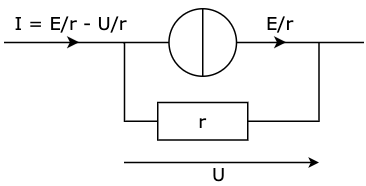
\includegraphics[width=\textwidth]{graphs/Norton}
            \centering
            \caption{Norton}
            \label{fig:courbe2}
        }
    \end{figure}

    On peut passer d'une représentation à une autre pour simplifier les résistances d'un circuit.\\


    \section{Méthodes de résolution}\label{sec:methodes-de-resolution}

    \subsection{Équations de résolution}\label{subsec:equations-de-resolution}

    Si on a $b$ branches, il va falloir $b$ équations pour déterminer tous les courants.\\
    La loi des noeuds nous donne $n-1$ équations, où $n$ est le nombre de noeuds.\\
    On établit donc $b - n + 1$ équations aux mailles pour déterminer toutes les intensités.

    \subsection{Transfiguration du réseau}\label{subsec:transfiguration-du-reseau}

    Deux sources de tension en série ou de courant en parallèle peuvent être simplifiées en appliquant la loi des mailles ou des noeuds.\\

    Deux résistances en séries peuvent être simplifiées en une seule résistance où $R_{eq} = R_1 + R_2$.\\
    En parallèle, c'est les intensités qui s'ajoutent donc $\dfrac{1}{R_{eq}} = \dfrac{1}{R_1} + \dfrac{1}{R_2}$, soit $R_{eq} = \dfrac{R_1 R_2}{R_1 + R_2}$.\\
    Si $R_1 = R_2$, alors $R_{eq} = \dfrac{R_1}{2}$.\\


    \section{Bilans de puissance}\label{sec:bilans-de-puissance}

    La puissance vaut toujours $P = UI$, mais sa signification dépend de la convention utilisée.


    \chapter{Circuits en régime transitoire}\label{ch:circuits-en-regime-transitoire}


    \section{Effet capacitif d'ordre 1}\label{sec:effet-capacitif-d'ordre-1}

    \subsection{Condensateur}\label{subsec:condensateur}

    Il s'établit un équilibre entre la charge du condensateur et la tension à ses bornes : $q = C u_c$.\\

    On a $i_c = \dfrac{\re d q}{\re d t} = C \dfrac{\re d u_c}{\re d t}$.\\
    $\rightarrow$ force la tension à être continue, car $i_c$ ne peut pas être infini.\\

    \subsection{Caractérisation du régime transitoire}\label{subsec:caracterisation-du-regime-transitoire}

    Tension de la forme : $u_c(t) = A e^{-\dfrac{t}{\tau}} + u_p$.\\

    $\tau$ caractérise la durée d'existence du régime transitoire.\\
    On peut le déterminer quantitativement :
    \begin{itemize}
        \item Pente à l'origine $\dfrac{u_p}{\tau} \cdot x = u_p \iff x = \tau$ :\\
        on regarde la distance horizontale, à la hauteur finale de la tension.
        \item Hauteur à $63\%$ :\\
        on regarde après quelle durée la tension est à $63\%$ de sa valeur finale.
    \end{itemize}

    \subsection{Analyse énergétique}\label{subsec:analyse-energetique}

    On associe une énergie à un condensateur : $E_c = \dfrac{1}{2} C u_c^2$.\\
    La puissance reçue par le condensateur est donc $P = \dfrac{\re d E_c}{\re d t} = C u_c \dfrac{\re d u_c}{\re d t}$.\\


    \section{Effet inductif d'ordre 1}\label{sec:effet-inductif-d'ordre-1}

    \subsection{Bobine}\label{subsec:bobine}

    Tension et courant sont liés par la relation : $u_L = L \dfrac{\re d i_L}{\re d t}$.\\
    $\rightarrow$ force le courant à être continue, car $u_L$ ne peut pas être infini.\\

    \subsection{Analyse énergétique}\label{subsec:analyse-energetique-2}

    On associe une énergie à une bobine : $E_L = \dfrac{1}{2} L i_L^2$.\\
    La puissance reçue par la bobine est donc $P = \dfrac{\re d E_L}{\re d t} = L i_L \dfrac{\re d i_L}{\re d t}$.\\


    \chapter{Régime sinusoïdal}\label{ch:regime-sinusoidal}


    \section{Introduction et définitions}\label{sec:introduction-et-definitions}

    \twoCol[53]{

        \subsection{Caractéristiques d'un signal sinusoïdal}\label{subsec:caracteristiques-d'un-signal-sinusoidal}

        \begin{itemize}
            \item Régime continu (DC) : I et U constates.
            \item Régime alternatif (AC) : souvent sinusoïdal
        \end{itemize}
        \vspace{10pt}
        On a donc $u(t) = U_m \sin(\omega t + \varphi)$ :
        \vspace{5pt}
        \begin{itemize}
            \item Amplitude $U_m$ : $U_{eff} = \dfrac{U_m}{\sqrt 2}$ et $U_{c-c}$ = $2 \times U_m$.
            \item Pulsation ou fréquence angulaire $\omega = 2\pi f = \dfrac{2\pi}{T}$.
            \item Phase $\omega t + \varphi$.
            \item Phase à l'origine $-\frac{\pi}{2} \le \varphi \le \frac{\pi}{2}$.
        \end{itemize}
    }{
        \subsection{Comparaison de tensions (ou intensités)}\label{subsec:comparaison-de-tensions-(ou-intensites)}

        En régime sinusoïdal forcé, $u(t)$ et $i(t)$ ont généralement la même fréquence que le générateur.
        On compare alors les amplitudes et les déphasages.\\

        Déphasage de $u_1$ par rapport à $u_2$ : $\Delta\varphi = \varphi_1 - \varphi_2$.
        (Positif si $u_1$ est en avance sur $u_2$).
    }

    \subsection{Représentation de Fresnel (diagramme de phase)}\label{subsec:representation-de-fresnel-(diagramme-de-phase)}

    $\Rightarrow$ Met en évidence les liens entre tension et courant en régime sinusoïdal.

    \vspace{5pt}
    On dessine des vecteurs par rapport à une référence de phase : $\varphi_i$ (série) ou $\varphi_u$ (dérivation) :
    \begin{itemize}
        \item Norme des vecteurs : $U_m$ ou $I_m$ (ou valeur efficace).
        \item Angle des vecteurs : $\varphi_u$ ou $\varphi_i$ (par rapport à la référence).
    \end{itemize}
    \vspace{5pt}
    Lorsqu'on fait la loi des mailles (ou des noeuds), on additionne alors les vecteurs.

    \subsection{Notation complexe associée}\label{subsec:notation-complexe-associée}

    La notation complexe n'a pas de sens physique.
    Module = amplitude, argument = phase.\\
    On s'intéressera uniquement à la partie réelle si $\cos$ ou imaginaire si $\sin$.\\

    $u(t) = U_m \cos(\omega t + \varphi)$ = \Re($U_m e^{j(\omega t + \varphi_u)}$)

%    Amplitude complexe : $\underline{U_m} = U_m e^{j\varphi_u}$ \quad On a donc $\underline{u}(t) = \underline{U_m} e^{j\omega t}$.


    \section{Impédances complexes}\label{sec:impedances-complexes}

    Impédance en convention récepteur : $\underline{z} = \dfrac{\underline{u}}{\underline{i}} = \dfrac{U_m}{I_m} e^{j(\varphi_u - \varphi_i)}$.\\

    \begin{itemize}
        \item Module de $\underline{z}$ : donne le rapport d'amplitude entre tension et courant.
        \item Argument de $\underline{z}$ : déphasage ($\varphi_u - \varphi_i$).
    \end{itemize}
    \\ \vspace{7pt}\\
    Impédances courantes :
    \begin{itemize}
        \item Résistance : $z = R$ (réel donc déphasage nul).
        \item Condensateur : $\underline{z} = \dfrac{-j}{C \omega}$ (imaginaire pur négatif donc déphasage de $-\frac{\pi}{2}$).
        \item Bobine : $\underline{z} = jL \omega$ (imaginaire pur positif donc déphasage de $\frac{\pi}{2}$).
    \end{itemize}


    \section{Lois en régime sinusoidal forcé}\label{sec:lois-en-regime-sinusoidal-force}

    Les lois de Kirchhoff sont toujours valables, mais bien uniquement avec les $u(t)$ et les $i(t)$.\\

    Les impédances s'additionnent en série et leurs inverse s'additionnent en parallèle.\\

    On a toujours l'équivalence Thévenin/Norton :\\
    $\underline{u} = \underline{e} - \underline{z} \underline{i} \iff \underline{i} = \dfrac{\underline{e}}{\underline{z}} - \dfrac{\underline{u}}{\underline{z}}$


    \chapter{Puissance en régime sinusoïdal}\label{ch:puissance-en-regime-sinusoidal}


    \section{Définitions}\label{sec:definitions}

    \underline{Puissance instantanée :} dépend du temps.
    On choisit $\varphi_i = 0$ et $\varphi_u \neq 0$ (ou l'inverse).\\
    On note alors $\varphi$ le déphasage de $u$ par rapport à $i$.\\

    $p(t)$ $= U_{m} I_{m} \cos(\omega t) \cos(\omega t + \varphi)$\\
    \phantom{$p(t)$ }$= U_{eff} I_{eff} \cos(\varphi) + U_{eff} I_{eff} \cos(2\omega t + \varphi)$\\

    Le premier terme ne dépend pas du temps : c'est la \underline{puissance active} (ou moyenne).\\
    $U_{eff} I_{eff}$ est la puissance apparente, et $\cos(\varphi_u)$ le facteur de puissance.\\

    Le second terme dépend du temps et a une période doublée.


    \section{Puissance des dipôles usuels}\label{sec:puissance-des-dipoles-usuels}

    \subsection{Résistance}\label{subsec:resistance}

    $\varphi_u = \varphi_i$\\
    $p(t) = U_{eff} I_{eff} + U_{eff} I_{eff} \cos(2 \omega t) \ge 0$

    \subsection{Condensateur}\label{subsec:condensateur-2}

    $\varphi_u - \varphi_i = - \dfrac{\pi}{2}$\\
    $p(t) = 0 + U_{eff} I_{eff} \cos\left(2 \omega t - \frac{\pi}{2}\right)$

    \subsection{Bobine idéale}\label{subsec:bobine-ideale}

    $\varphi_u - \varphi_i = \dfrac{\pi}{2}$\\
    $p(t) = 0 + U_{eff} I_{eff} \cos\left(2 \omega t + \frac{\pi}{2}\right)$


    \chapter{Filtres électroniques}\label{ch:filtres-electroniques}

    \section{Qu'est-ce qu'un filtre ?}\label{sec:quest-ce-qu-un-filtre}

    C'est un quadripôle, un circuit avec des dipôles passifs (résistances, condensateurs et/ou bobines).\\
    Laisse passer certaines fréquences et en atténue plus ou moins d'autres.

    \section{Fonction de transfert : définitions}\label{sec:fonction-de-trandfert-definitions}

    Fonction complexe, $\underline{H}(j\omega) = \dfrac{\underline{u}_s}{\underline{u}_e} = \dfrac{U_s_m}{U_e_m} e^{\varphi_{u_s} - \varphi_{u_e}}$\\

    \begin{itemize}
        \item Module de $H$ : gain $G(\omega) = \dfrac{U_s_m}{U_e_m}$
        \item Argument de $H$ : déphasage $\varphi(\omega) = \varphi_{u_s} - \varphi_{u_e}$
    \end{itemize}

    \section{Diagramme de Bode}\label{sec:diagramme-de-bode}

    \underline{Abscisse :} $f$ ou $\omega$ (logarithmique).\\
    \underline{Ordonnée :} $G_{dB}$ ou $\varphi$ (linéaire).\\
    On parle de diagramme de bode en Gain ou en Phase.\\

    $G_{dB} = 20 \times \log(G)$

    \section{Fréquence(s) de coupure}\label{sec:frequence-s-de-coupure}

    Soit $\omega_C$ la pulsation de coupure.\\
    Le filtre coupe si $G(j\omega) < G(\omega_C)$ et laisse passer, si $G(j\omega) > G(\omega_C)$
    \begin{align*}
        G(\omega_C) &= \dfrac{G_{\max}}{\sqrt{2}}\\
        G_{dB}(\omega_C) &= G_{dB_\re{max}}(\omega_C) - 3\ dB
    \end{align*}

    Bande passante : ensemble des fréquences que le filtre laisse passer.

    \section{Types de filtres usuels}\label{sec:types-de-filtres-usuels}

    \begin{itemize}
        \item Passe bas : $G_{dB} = 0$ puis décroissant (LR ou RC).
        \item Passe haut : $G_{dB}$ croissant puis constant $= 0$ (RL ou CR).
        \item Passe bande : $G_{dB}$ croissant, constant $= 0$ puis décroissant (condensateur et bobine en série).
        \item Coupe bande : $G_{dB}$ constant $= 0$, constant $< 0$, constant $= 0$ (condensateur et bobine en parallèle).
    \end{itemize}


\end{document}
